\chapter{How Complex Numbers Generate Structure}
\label{chap:VII_complex_structure}

Complex numbers are not only an extension of the concept of number,
but a space in which surprisingly rich structures can arise from simple rules.
This becomes especially clear in iterated mappings:
a single prescription is applied again and again to its own result,
thereby generating orbits, boundaries, and forms
that reach far beyond the individual calculation scheme.

This chapter shows
how stability, divergence, and boundary structures arise
from the iteration of complex numbers,
how the Mandelbrot set can be read as a map of parameter space,
and why Julia sets make local dynamics visible.
In the end, it becomes clear
that nature is not being depicted here;
rather, structure is generated from mathematics itself.

% =====================================================
% 7.1 Iteration as a Mathematical Principle
% =====================================================

\subsection{Iteration as a Mathematical Principle}

\index{dynamical system}
\index{mapping}
\index{orbit}

Iteration is one of the simplest and at the same time most powerful principles of mathematics:
a prescription is applied, and then its result is subjected to the same prescription again.
In this way, a sequence of states arises from a single rule.
This is exactly where what may be called \emph{structure from mathematics} begins.

Formally, iteration is the repeated application of a mapping $f$:
\[
z_0,\quad z_1=f(z_0),\quad z_2=f(z_1)=f(f(z_0)),\quad \ldots,\quad z_{n+1}=f(z_n).
\]
Thus a single starting value $z_0$ generates an entire orbit in state space.

\subsubsection*{A Simple Numerical Example}

Let us take a particularly simple function on the real numbers:
\[
f(x)=\frac12 x + 1.
\]
We start with $x_0=0$ and repeatedly apply the same prescription:
\[
\begin{aligned}
	x_1 &= f(x_0)=1,\\
	x_2 &= f(x_1)=1{,}5,\\
	x_3 &= f(x_2)=1{,}75,\\
	x_4 &= 1{,}875,\\
	x_5 &= 1{,}9375,\\
	x_6 &= 1{,}96875.
\end{aligned}
\]
One immediately sees:
the sequence approaches a fixed number, namely $2$.
This number is called a \emph{fixed point}, because
\[
f(2)=2.
\]
\index{fixed point}

This point of view is decisive:
numbers become states,
and the function $f$ becomes the dynamics.
Thus iteration is already a dynamical system
in the purest and most abstract sense.

\begin{MathBox}[Terms: Orbit and Fixed Point]
	\phantomsection\label{box:orbit}
	Let $f:\mathbb{C}\to\mathbb{C}$ be given, and let $z_0\in\mathbb{C}$ be a starting value.
	The iteration is
	\[
	z_{n+1}=f(z_n)\qquad (n=0,1,2,\dots).
	\]
	The sequence $(z_0,z_1,z_2,\dots)$ is called the \emph{orbit} of $z_0$.
	A point $z^\ast$ is called a \emph{fixed point} if
	\[
	f(z^\ast)=z^\ast
	\]
	holds.
\end{MathBox}

\subsubsection*{Why Complex Numbers Are Special Here}
\index{complex number}
\index{complex plane}

On the real axis, an iteration proceeds along a number line.
In the complex plane, by contrast, it moves in two dimensions.
This step alone changes the situation fundamentally:
orbits can circle,
spiral,
form boundaries,
generate islands,
and develop finely branched edges.
A calculation rule becomes geometry.

For the later images of the Mandelbrot and Julia sets,
one family of mappings is already sufficient at its core:
\[
f_c(z)=z^2+c \qquad (z,c\in\mathbb{C}).
\]
One starts with a value $z_0$
and then follows the further iteration.
The guiding question is simple,
but far-reaching:
\emph{Does the orbit remain bounded, or does it escape to infinity?}

\subsubsection*{Brief Conclusion}

\begin{itemize}
	\item Iteration means applying the same prescription repeatedly.
	\item This generates orbits with qualitatively different behavior: stable, periodic, or divergent.
	\item In the complex plane, this behavior becomes directly visible as form.
\end{itemize}

This prepares the next step:
What exactly does ``bounded'' mean,
what does ``divergent'' mean,
and why is the actual structure located precisely at the boundary between the two?

% =====================================================
% 7.2 Stability, Divergence, and Boundary Cases
% =====================================================

\subsection{Stability, Divergence, and Boundary Cases}

\index{boundary case}
\index{boundedness}
\index{absolute value}

When we consider an iteration $z_{n+1}=f(z_n)$, the central question is not:
``Which number comes next?''
Rather, it is:
\emph{What happens in the long run?}
Does the orbit remain within a bounded region, or does it run away?
This simple distinction separates stable from unstable dynamics.

\subsubsection*{Stability: Orbits Remain Nearby}

In the stable case, a starting value is robust:
small changes in the starting value may change the sequence,
but not its qualitative behavior.
One can imagine it this way:
the iteration draws orbits into a certain region
instead of driving them outward.
Typically, this involves convergence toward a fixed point or a periodic cycle.
\index{fixed point}

\subsubsection*{Divergence: Orbits Fly Away}

In the unstable case, the opposite happens:
the iteration amplifies deviations.
The sequence grows further and further in absolute value;
it ``escapes'' from every bounded region.
This is exactly the behavior we will later use as a criterion:
\emph{What flies away does not belong to the structure.}

\subsubsection*{Two Mini-Examples: Stable vs.\ Divergent}

\begin{figure}[h]
	\centering
	
	\begin{tikzpicture}
		\begin{axis}[
			width=0.46\textwidth,
			height=4.2cm,
			xlabel={$n$},
			ylabel={$x_n$},
			title={Stable: $x_{n+1}=\tfrac12 x_n+1$},
			ymin=0, ymax=2.1,
			xtick={0,1,2,3,4,5,6,7,8},
			ytick={0,0.5,1,1.5,2}
			]
			\addplot+[mark=*] coordinates {
				(0,0)
				(1,1)
				(2,1.5)
				(3,1.75)
				(4,1.875)
				(5,1.9375)
				(6,1.96875)
				(7,1.984375)
				(8,1.9921875)
			};
		\end{axis}
	\end{tikzpicture}
	\hfill
	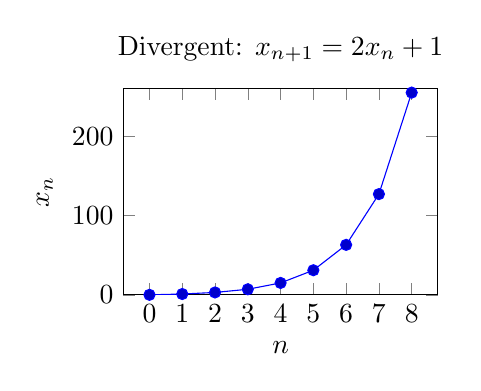
\begin{tikzpicture}
		\begin{axis}[
			width=0.46\textwidth,
			height=4.2cm,
			xlabel={$n$},
			ylabel={$x_n$},
			title={Divergent: $x_{n+1}=2x_n+1$},
			ymin=0, ymax=260,
			xtick={0,1,2,3,4,5,6,7,8}
			]
			\addplot+[mark=*] coordinates {
				(0,0)
				(1,1)
				(2,3)
				(3,7)
				(4,15)
				(5,31)
				(6,63)
				(7,127)
				(8,255)
			};
		\end{axis}
	\end{tikzpicture}
\end{figure}

\begin{DidacticBox}[Stable vs.\ Chaotic: Do Not Confuse Them]
	\phantomsection\label{box:stable}
	Stability does not mean ``boring,''
	and instability does not automatically mean ``random.''
	Chaotic orbits are deterministic as well,
	but they are sensitive to the smallest changes.
	For our purposes, the more robust guiding idea is sufficient at first:
	\emph{bounded} versus \emph{unbounded}.
	The boundary region between the two will later be the place of visible structure.
\end{DidacticBox}

\subsubsection*{Boundedness as a Criterion}

In the complex plane, it is especially natural to consider the \emph{absolute value} $|z_n|$.
We call an orbit \emph{bounded} if there exists a number $R>0$ such that
\[
|z_n|\le R \quad \text{for all } n.
\]
If no such $R$ exists, then the orbit runs off to infinity:
$|z_n|\to\infty$.

\begin{MathBox}[Bounded or Unbounded]
	\phantomsection\label{box:bounded}
	For the iteration $z_{n+1}=f(z_n)$, the orbit of $z_0$ is called \emph{bounded} if
	\[
	\exists\, R>0:\ \forall n\in\mathbb{N}\ \ |z_n|\le R.
	\]
	If this is not the case, the orbit is called \emph{unbounded} or divergent;
	typically, one then has $|z_n|\to\infty$.
\end{MathBox}

\subsubsection*{A Simple Complex Example: A Spiral Orbit Inside a Circle}

We consider the iteration
\[
z_{n+1}=a\,z_n,\qquad a=0{,}85\,e^{i\pi/5},\qquad z_0=2+i.
\]
Since $|a|=0{,}85<1$, for all $n$:
\[
|z_n|=|a|^n|z_0|\le |z_0|=:R=\sqrt{5}.
\]
The orbit therefore remains within the circle of radius $R$ and spirals toward $0$.

\subsubsection*{Two Iteration Steps for Understanding}

We write
\[
a=0{,}85e^{i\pi/5}=0{,}85(\cos36^\circ+i\sin36^\circ)
\approx 0{,}687664+i\,0{,}499617.
\]
With $z_0=2+i$, this gives
\begin{align*}
	z_1 &= a z_0\\
	&= (0{,}687664+i\,0{,}499617)(2+i)\\
	&= (2\cdot0{,}687664-0{,}499617)+i(0{,}687664+2\cdot0{,}499617)\\
	&\approx 0{,}876+i\,1{,}687.
\end{align*}
The next step is
\[
z_2=a z_1\approx (0{,}687664+i\,0{,}499617)(0{,}876+i\,1{,}687)
\approx -0{,}241+i\,1{,}598.
\]
One can already see:
each step rotates the point by $36^\circ$ and reduces the absolute value by the factor $0{,}85$.
In general,
\[
|z_n|=0{,}85^n|z_0|,\qquad \arg(z_n)=\arg(z_0)+n\frac{\pi}{5},
\]
so the orbit spirals toward $0$.

\begin{figure}[h]
	\centering
	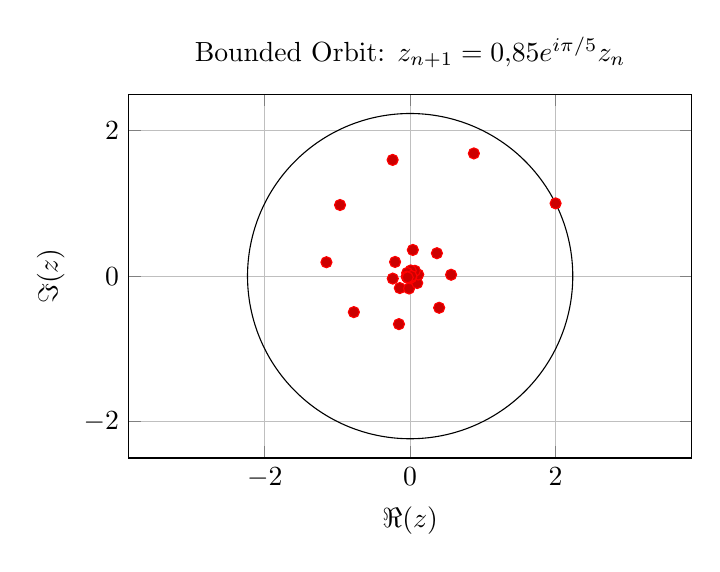
\begin{tikzpicture}
		\begin{axis}[
			axis equal,
			width=0.72\textwidth,
			height=6.2cm,
			xlabel={$\Re(z)$},
			ylabel={$\Im(z)$},
			title={Bounded Orbit: $z_{n+1}=0{,}85e^{i\pi/5}z_n$},
			xmin=-2.5, xmax=2.5,
			ymin=-2.5, ymax=2.5,
			grid=both
			]
			\addplot[domain=0:360, samples=361] ({sqrt(5)*cos(x)},{sqrt(5)*sin(x)});
			\addplot+[only marks, mark=*] coordinates {
				(2.000,1.000)
				(0.876,1.687)
				(-0.241,1.598)
				(-0.964,0.978)
				(-1.151,0.191)
				(-0.774,-0.495)
				(-0.154,-0.660)
				(0.399,-0.435)
				(0.563,0.019)
				(0.368,0.315)
				(0.037,0.360)
				(-0.207,0.195)
				(-0.239,-0.034)
				(-0.142,-0.164)
				(-0.015,-0.170)
				(0.097,-0.095)
				(0.111,0.022)
				(0.066,0.073)
				(0.008,0.078)
				(-0.041,0.044)
				(-0.048,-0.007)
				(-0.030,-0.026)
				(-0.005,-0.028)
				(0.015,-0.016)
				(0.017,0.002)
				(-0.034,-0.017)
			};
		\end{axis}
	\end{tikzpicture}
\end{figure}

\newpage
\noindent

\subsubsection*{The Boundary Case: The Actual Stage of Structure}

Now comes the decisive point for the whole chapter:
between clearly stable and clearly divergent lies a boundary region that is extremely sensitive.
Starting values that differ only minimally can end in completely different ways:
one orbit remains bounded, the other flies away.
This transition is not a side effect, but the center of the phenomenon.

This is precisely why sharp, frayed boundaries and seemingly infinite depth of detail arise later.
Not because we are modeling nature,
but because we are asking a boundary question.

\subsubsection*{Extremely Sensitive: Minimal Change, Completely Different Behavior}

We consider the iteration
\[
z_{n+1}=z_n^2,
\]
that is, the quadratic map $f(z)=z^2$.
Here the boundary case can be understood completely:
\emph{The boundary between bounded and unbounded is the unit circle $|z|=1$.}
This already shows what later appears in a much more complicated form
in Mandelbrot and Julia sets:
a boundary region decides between ``stays inside'' and ``flies away.''

We choose two almost identical starting values:
\[
z_0=0{,}99 \quad (\text{just inside}), 
\qquad z_0=1{,}01 \quad (\text{just outside}).
\]

\begin{figure}[h]
	\centering
	
	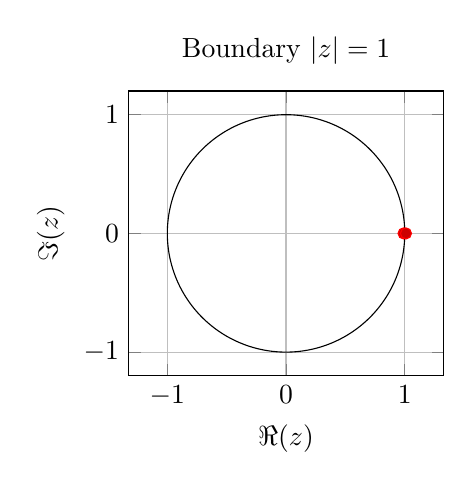
\begin{tikzpicture}
		\begin{axis}[
			axis equal,
			width=0.46\textwidth,
			height=5.2cm,
			xlabel={$\Re(z)$},
			ylabel={$\Im(z)$},
			title={Boundary $|z|=1$},
			xmin=-1.2, xmax=1.2,
			ymin=-1.2, ymax=1.2,
			grid=both
			]
			\addplot[domain=0:360, samples=361] ({cos(x)},{sin(x)});
			\addplot+[only marks, mark=*] coordinates {(0.99,0) (1.01,0)};
		\end{axis}
	\end{tikzpicture}
	\hfill
	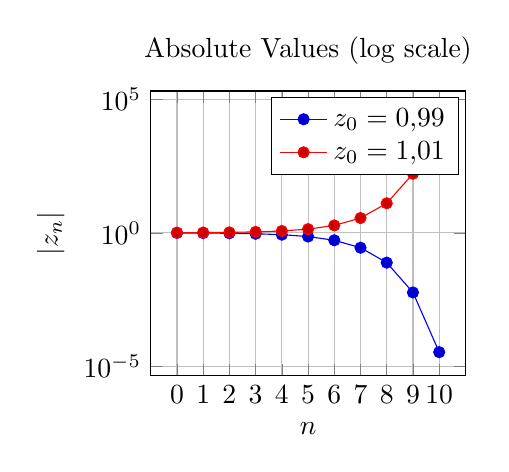
\begin{tikzpicture}
		\begin{axis}[
			width=0.46\textwidth,
			height=5.2cm,
			xlabel={$n$},
			ylabel={$|z_n|$},
			title={Absolute Values (log scale)},
			ymode=log,
			log basis y={10},
			xtick={0,1,2,3,4,5,6,7,8,9,10},
			grid=both
			]
			\addplot+[mark=*] coordinates {
				(0,0.99)
				(1,0.9801)
				(2,0.96059601)
				(3,0.9227446944)
				(4,0.8514577711)
				(5,0.7249803360)
				(6,0.5255964875)
				(7,0.2762516677)
				(8,0.0763149839)
				(9,0.0058239768)
				(10,0.0000339187)
			};
			\addlegendentry{$z_0=0{,}99$}
			
			\addplot+[mark=*] coordinates {
				(0,1.01)
				(1,1.0201)
				(2,1.04060401)
				(3,1.0828567056)
				(4,1.1725786449)
				(5,1.3749406785)
				(6,1.8904618695)
				(7,3.5738460800)
				(8,12.7723758032)
				(9,163.1335836586)
				(10,26612.5661173053)
			};
			\addlegendentry{$z_0=1{,}01$}
		\end{axis}
	\end{tikzpicture}
	
	\caption{Boundary case for $z_{n+1}=z_n^2$: inside the unit circle, orbits remain bounded; outside it, they diverge. Even a minimal change in the starting value can completely flip the behavior.}
\end{figure}

\subsubsection*{Preparation for the Quadratic Map $z^2+c$}
\index{quadratic map}

For the family $f_c(z)=z^2+c$, there will even be a practical criterion:
if the absolute value of an orbit eventually becomes large enough,
then it is certain that it will continue to grow and escape.
Thus ``belongs'' versus ``does not belong'' can be decided computationally.
Now the idea becomes a map:
For which parameters $c$ does the orbit of $z_0=0$ remain bounded?
Exactly this set is the Mandelbrot set.

% =====================================================
% 7.3 The Mandelbrot Set as a Map
% =====================================================

\subsection{The Mandelbrot Set as a Map}
\label{sec:VII-7-3}
\index{Mandelbrot set}
\index{parameter space}
\index{boundedness}
\index{escape time}
\index{escape radius}
\index{fractal}

\textbf{Guiding question:} \emph{How can the Mandelbrot set be read like a map -- and what do ``land,'' ``sea,'' and ``coast'' mean mathematically?}

The Mandelbrot set is not the trajectory of a single iteration.
It is a \emph{map in parameter space}:
each point \(c\) in the complex plane stands for its own iteration system.
The image therefore does not arrange the values of one single sequence \(z_n\),
but entire \emph{systems according to their behavior}.

\begin{MathBox}[Definition: Map in Parameter Space]
	\phantomsection\label{box:map}
	We consider the iteration
	\[
	z_{n+1}=z_n^2+c,\qquad z_0=0,\qquad c\in\mathbb{C}.
	\]
	The \textbf{Mandelbrot set} is the set of all parameters \(c\)
	for which the sequence \(\{z_n\}\) remains \textbf{bounded}:
	\[
	\mathcal{M}=\{\,c\in\mathbb{C}\mid \sup_n |z_n|<\infty\,\}.
	\]
\end{MathBox}

\begin{DidacticBox}[The Most Common Misconception]
	\phantomsection\label{box:misconception}
	In the graphic, the coordinate is \textbf{not} \(z\),
	but the parameter \(c\).
	For \emph{each} image point, the same iteration is started
	(always with \(z_0=0\)),
	but each time with a different \(c\).
	That is why the image is a \textbf{map}:
	each point corresponds to its own small dynamical ``universe.''
\end{DidacticBox}

\subsubsection*{Land, Sea, and Coast}

The map metaphor is not only intuitive,
but mathematically precise:

\begin{itemize}
	\item \textbf{Land} (inside, often black): The sequence \(\{z_n\}\) remains bounded, so \(c\in\mathcal{M}\).
	\item \textbf{Sea} (outside, usually colored): The sequence escapes, so it diverges.
	\item \textbf{Coast} (the boundary): Transition region where the smallest changes in \(c\) can flip the behavior.
\end{itemize}

As soon as, in the iteration \(z_{n+1}=z_n^2+c\), a value with \(|z_n|>2\) occurs,
divergence is certain.
This number \(2\) is called the \emph{escape radius}.
Outside the Mandelbrot set, the coloring usually shows the \emph{escape time},
that is, the number of iterations
until \(|z_n|>2\) is reached.
This is a visualization tool,
not part of the actual definition.

\subsubsection*{The Boundary as the Stage of Structure}

The actual core of the Mandelbrot set
lies neither simply in the inside nor in the outside,
but on its \textbf{boundary}.
There the entire complexity is concentrated.
Tiny changes of the parameter \(c\)
decide whether the orbit remains bounded or escapes.
Precisely in this transition region,
new structures appear again and again when one zooms in --
this is the characteristic feature of fractal geometry.

\begin{figure}[htbp]
	\centering
	
\includegraphics[width=0.88\linewidth]{Bilder/Mandelbrot.png}
	\caption{The Mandelbrot set as a map in the parameter space \(c\):
		bounded inside (land),
		escape-time coloring outside (sea),
		and on the boundary a structurally rich ``coastal region.''}
	\label{fig:mandelbrot_landkarte}
\end{figure}

\subsubsection*{Key Points}

\begin{itemize}
	\item The Mandelbrot set is an image of the \textbf{parameter space}: each point stands for its own iteration system.
	\item \textbf{Inside} means: the orbit of \(z_0=0\) remains bounded.
	\item \textbf{Outside} means: the orbit escapes; the colors usually show the escape time.
	\item The \textbf{boundary} is the decisive region: this is where all the depth of detail resides.
\end{itemize}

A detailed and reproducible generation of the Mandelbrot graphic
-- from the assignment of pixels to \(c\)-values
through iteration to escape time and coloring --
can be found in Appendix~\ref{app:mandelbrot-rendering}.

This prepares the next step:
whereas the Mandelbrot set is a map of \emph{parameter space},
Julia sets show the dynamics in \emph{state space}.
For a fixed \(c\), they make visible
which starting values \(z_0\) remain bound
and which escape.

% =====================================================
% 7.4 Julia Sets: Local Dynamics and Structure
% =====================================================

\subsection{Julia Sets: Local Dynamics and Structure}
\label{sec:julia-sets}
\index{Julia set}
\index{complex dynamics}
\index{Mandelbrot set}

\textbf{Guiding question:} What happens \emph{locally} in \(z\)-space when the parameter \(c\) is fixed -- and why do such different, often fractal boundaries arise?

The Mandelbrot set from Section~\ref{sec:VII-7-3} is a \emph{map of parameter space}:
each point \(c\) stands for its own iteration system.
Julia sets are the corresponding \emph{maps of state space}:
for a \emph{fixed} \(c\), one considers the orbit of a starting value \(z_0\) under iteration.
Thus the question
``Where is \(c\)?''
becomes the question:
``Which starting values \(z_0\) remain bound -- and which escape?''

\begin{MathBox}[Definition: Iteration, Filled Julia Set, Julia Boundary]
	\phantomsection\label{box:iteration}
	We consider the quadratic iteration
	\[
	z_{n+1}=f_c(z_n)=z_n^2+c \qquad (c\in\mathbb{C}\ \text{fixed}).
	\]
	\begin{itemize}
		\item The \emph{orbit} of \(z_0\) is the sequence \((z_n)_{n\ge 0}\).
		\item The \emph{filled Julia set} is
		\[
		K_c=\{z_0\in\mathbb{C}\mid (z_n)\ \text{remains bounded}\}.
		\]
		\item The \emph{Julia set} is the boundary
		\[
		J_c=\partial K_c.
		\]
	\end{itemize}
	Intuitively:
	\(K_c\) consists of the starting values that do not escape,
	and \(J_c\) is the sharp, fractal boundary between bound and divergent.
\end{MathBox}

\subsubsection*{Local Dynamics: Stability, Escape, and Sensitive Boundaries}
\index{stability}
\index{divergence}

For many starting values, the behavior is decided quickly:
either the sequence remains within a bounded region,
or it rapidly grows beyond all bounds.
The surprising part is not the escape itself,
but the geometry of the dividing line.
The boundary \(J_c\) is typically extremely rugged and sensitive.
A minimal difference in \(z_0\)
can decide
whether the orbit remains bound or escapes.

\subsubsection*{Three Simple Examples for Orientation}

One does not need to know many formulas --
three examples are enough to understand the basic pattern:

\begin{itemize}
	\item \textbf{\(c=0\):} Then \(z_{n+1}=z_n^2\).
	The filled Julia set \(K_0\) is the closed unit disk,
	and \(J_0\) is its boundary, the unit circle.
	Here the boundary is smooth and not yet fractal.
	\index{unit circle}
	\item \textbf{\(c=-1\):} The classical ``Basilica'' image arises:
	two large lobes, clearly recognizable,
	but already with a highly complex boundary.
	\index{Basilica}
	\item \textbf{\(c\) close to the boundary of the Mandelbrot set:} Julia sets then often become especially delicate.
	Dendrites and dust-like structures appear,
	and the local dynamics reacts with particular sensitivity.
\end{itemize}

\begin{HistoryBox}[Historical Context: Julia and Fatou]
	\phantomsection\label{box:julia}
	The systematic investigation of complex iterations began around 1918 to 1920 with Gaston Julia and Pierre Fatou.
	The central concepts of the stable region, the Fatou set, and the chaotic boundary, the Julia set, come from this period.
	This is an impressive example of how pure mathematics became the visual language of modern fractals decades later.
\end{HistoryBox}

\subsubsection*{The Key Connection Between Julia and Mandelbrot}
\index{Mandelbrot set}

The Mandelbrot set is not only a beautiful image,
but a \emph{classification map}.
It assigns to each parameter \(c\)
the type of the corresponding Julia set.
This is exactly where parameter space (\(c\))
and state space (\(z\)) meet directly.

\subsubsection*{Connection Between \(c\) and the Geometry of \(J_c\)}

For the iteration \(z_{n+1}=z_n^2+c\), the following holds:
if \(c\) lies \emph{inside} the Mandelbrot set,
then the filled Julia set \(K_c\),
and therefore also its boundary \(J_c\), is connected.
If \(c\) lies \emph{outside},
then \(J_c\) typically breaks apart
into many separate islands,
that is, into a kind of ``dust.''

This makes the idea from Section~\ref{sec:VII-7-3} precise:
the Mandelbrot set does not tell us
\emph{what} a Julia set looks like in detail,
but it immediately tells us
whether to expect a connected structure
or a disintegrating dust.

\subsubsection*{How Are the Images Generated?}

For visualization, one tests in practice for each pixel starting value \(z_0\)
whether the orbit escapes
and after how many steps this happens.
The color then typically encodes the \emph{escape time}
or a smoothed variant of it.
The clean and reproducible rendering idea
-- iteration, stopping criterion, and color assignment --
is documented in detail in the appendix;
see Appendix~\ref{app:mandelbrot-rendering}.

\newpage
\noindent
\subsubsection*{Example 1: Smooth Boundary Case (\(c=0\))}
\index{Julia set}
\index{unit circle}

Here the dynamics is especially intuitive:
the boundary is smooth.
The Julia set is the unit circle;
inside it, the orbits remain bound,
and outside it, they escape.

\begin{figure}[htbp]
	\centering
	
\includegraphics[width=0.82\textwidth]{Bilder/Julia_0.png}
	\caption{Julia set for \(c=0\): \(J_c\) is the unit circle.}
	\label{fig:julia-c0}
\end{figure}

\newpage
\noindent
\subsubsection*{Example 2: Connected but Fractal (\(c=-1\))}
\index{Basilica}

Despite its clear overall form, the boundary is already highly complex:
bound and escaping starting values
lie arbitrarily close to one another there.

\begin{figure}[htbp]
	\centering
	
\includegraphics[width=0.82\textwidth]{Bilder/Julia-1.png}
	\caption{Julia set for \(c=-1\) (``Basilica''): connected, but with a fractal boundary.}
	\label{fig:julia-cminus1}
\end{figure}

\newpage
\noindent
\subsubsection*{Example 3: Outside the Mandelbrot Set (``Dust'')}
\index{Mandelbrot set}
\index{Cantor dust}

Outside the Mandelbrot set,
\(J_c\) typically breaks apart into many separate islands:
the boundary is then no longer connected,
but appears as scattered ``dust.''

\begin{figure}[htbp]
	\centering
	
\includegraphics[width=0.82\textwidth]{Bilder/Julia-2.png}
	\caption{Julia set for a \(c\) outside the Mandelbrot set: disintegrating ``dust.''}
	\label{fig:julia-c2}
\end{figure}

% =====================================================
% 7.5 Self-Similarity and Scale Invariance
% =====================================================

\subsection{Self-Similarity and Scale Invariance}
\label{sec:7.5}
\index{self-similarity}
\index{scale invariance}
\index{fractal dimension}
\index{box-counting dimension}

\textbf{Guiding question:} Why do similar structures keep appearing when one zooms into Mandelbrot and Julia sets -- and what does this mean mathematically?

For many objects of classical geometry, the image eventually becomes \emph{simpler} when magnified:
a circular line remains smooth, and a polygon shows straight edges.
For fractal sets, the opposite is true:
magnification does not produce less visible structure, but more.
This behavior is described by the terms \emph{self-similarity} and \emph{scale invariance}.

\subsubsection*{Self-Similarity: Recurrence of Structure}

In everyday language, self-similarity often means a direct copy:
a pattern appears again, only on a smaller scale.
In dynamically generated fractals such as Mandelbrot and Julia sets,
this is usually not the case in a strict sense.
Instead, one observes a \emph{quasi-self-similar} recurrence:
certain motifs -- such as bulbs, filaments, spiral forms, or so-called ``seahorse'' structures --
appear again on different scales,
though not as perfect duplicates.

\begin{DidacticBox}[Self-Similarity Does Not Mean: Identical Copy]
	\phantomsection\label{box:copy}
	\small
	In iterated complex mappings, self-similarity is often \emph{qualitative}:
	when zooming in, similar forms and stability islands appear again,
	but usually with distortions, rotations, or slight variations.
	The decisive point is therefore not ``copy and paste,''
	but:
	\emph{the type of structure is preserved.}
\end{DidacticBox}

Nevertheless, it is useful to know the exact idea briefly.
In classical fractal geometry, a set \(S\) is called self-similar
if it consists of scaled-down copies of itself.
Formally, similarity mappings \(f_k\) then exist such that
\[
S=\bigcup_{k=1}^m f_k(S),\qquad
f_k(z)=r_k e^{i\theta_k}z+t_k,\quad 0<r_k<1.
\]
This is the principle of the Koch curve or the Sierpiński triangle.
For Mandelbrot and Julia sets, the situation is more subtle:
self-similarity does not arise from a fixed \emph{construction plan},
but from the \emph{dynamics} of the iteration.

\subsubsection*{Scale Invariance: No Characteristic Size}

Scale invariance means
that there is no distinguished length scale
at which the structure suddenly disappears.
If one magnifies by a factor \(\lambda>0\),
\[
z \mapsto \lambda z,
\]
the structure does not necessarily remain identical,
but it remains of the same type.
Precisely this is the visual core of many fractals:
even on smaller and smaller scales, boundary structure remains present.

\subsubsection*{Why Does This Occur in the Mandelbrot Set?}

The Mandelbrot set is a map of the stability of the iteration
\[
z_{n+1}=z_n^2+c.
\]
For parameters \(c\) \emph{inside} the Mandelbrot set,
the orbit of \(z_0=0\) remains bounded;
outside, it diverges.
The \emph{boundary} of the set marks the transition between stability and divergence.
Such transitions are precisely the places
where dynamics becomes sensitive
and generates new structure on many scales.

When one zooms into these boundary regions,
so-called \emph{baby Mandelbrots} appear again and again,
that is, small Mandelbrot-like substructures.
Didactically, this is the decisive point:

\begin{quote}
	\emph{Self-similarity is the geometric signature of dynamics at the edge of stability.}
\end{quote}

Thus one sees not only an impressive image,
but a recurring order:
stable period windows are embedded
in a delicate and sensitive boundary fabric.

\subsubsection*{Julia Sets: Structure Depends on the Parameter}

The Julia set belongs to the same iteration,
but for a fixed \(c\):
\[
f_c(z)=z^2+c.
\]
A fundamental connection is:

\begin{itemize}
	\item If \(c\) lies \emph{inside} the Mandelbrot set, then the corresponding Julia set is \emph{connected}.
	\item If \(c\) lies \emph{outside}, then the Julia set breaks apart into ``dust,'' that is, into a Cantor-like set.
\end{itemize}

This makes understandable
why Julia sets, when zoomed into, often also show self-similar motifs,
but vary strongly in appearance:
the parameter \(c\) determines
whether one obtains a closed, filament-like structure
or a disintegrating point ensemble.

\subsubsection*{Making Scale Invariance Measurable: Fractal Dimension}

The fact that an object carries detail on many scales
can also be captured quantitatively.
A robust method is \emph{box counting}:
one covers the boundary set under investigation with squares of side length \(\varepsilon\)
and counts
how many boxes \(N(\varepsilon)\) are needed.

\begin{figure}[H]
	\centering
	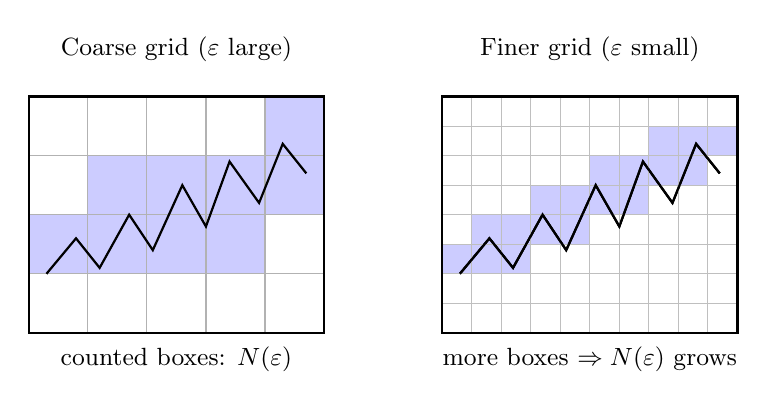
\begin{tikzpicture}[scale=0.75]
		\begin{scope}[shift={(0,0)}]
			\node at (2.5,4.8) {\small Coarse grid (\(\varepsilon\) large)};
			\draw[thick] (0,0) rectangle (5,4);
			\draw[gray!60, step=1] (0,0) grid (5,4);
			\draw[thick]
			(0.3,1.0) -- (0.8,1.6) -- (1.2,1.1) -- (1.7,2.0)
			-- (2.1,1.4) -- (2.6,2.5) -- (3.0,1.8) -- (3.4,2.9)
			-- (3.9,2.2) -- (4.3,3.2) -- (4.7,2.7);
			\fill[blue!20] (0,1) rectangle (1,2);
			\fill[blue!20] (1,1) rectangle (2,2);
			\fill[blue!20] (1,2) rectangle (2,3);
			\fill[blue!20] (2,1) rectangle (3,2);
			\fill[blue!20] (2,2) rectangle (3,3);
			\fill[blue!20] (3,1) rectangle (4,2);
			\fill[blue!20] (3,2) rectangle (4,3);
			\fill[blue!20] (4,2) rectangle (5,3);
			\fill[blue!20] (4,3) rectangle (5,4);
			\draw[gray!60, step=1] (0,0) grid (5,4);
			\draw[thick] (0,0) rectangle (5,4);
			\draw[thick]
			(0.3,1.0) -- (0.8,1.6) -- (1.2,1.1) -- (1.7,2.0)
			-- (2.1,1.4) -- (2.6,2.5) -- (3.0,1.8) -- (3.4,2.9)
			-- (3.9,2.2) -- (4.3,3.2) -- (4.7,2.7);
			\node at (2.5,-0.45) {\small counted boxes: \(N(\varepsilon)\)};
		\end{scope}
		
		\begin{scope}[shift={(7,0)}]
			\node at (2.5,4.8) {\small Finer grid (\(\varepsilon\) small)};
			\draw[thick] (0,0) rectangle (5,4);
			\draw[gray!50, step=0.5] (0,0) grid (5,4);
			\foreach \x/\y in {
				0/1,0.5/1,0.5/1.5,
				1/1,1/1.5,1.5/1.5,
				1.5/2,2/1.5,2/2,
				2.5/2,2.5/2.5,3/2,
				3/2.5,3.5/2.5,3.5/3,
				4/2.5,4/3,4.5/3
			}{
				\fill[blue!20] (\x,\y) rectangle ++(0.5,0.5);
			}
			\draw[thick]
			(0.3,1.0) -- (0.8,1.6) -- (1.2,1.1) -- (1.7,2.0)
			-- (2.1,1.4) -- (2.6,2.5) -- (3.0,1.8) -- (3.4,2.9)
			-- (3.9,2.2) -- (4.3,3.2) -- (4.7,2.7);
			\draw[gray!50, step=0.5] (0,0) grid (5,4);
			\draw[thick] (0,0) rectangle (5,4);
			\draw[thick]
			(0.3,1.0) -- (0.8,1.6) -- (1.2,1.1) -- (1.7,2.0)
			-- (2.1,1.4) -- (2.6,2.5) -- (3.0,1.8) -- (3.4,2.9)
			-- (3.9,2.2) -- (4.3,3.2) -- (4.7,2.7);
			\node at (2.5,-0.45) {\small more boxes \(\Rightarrow N(\varepsilon)\) grows};
		\end{scope}
	\end{tikzpicture}
	\caption{Box-counting idea: one does not cover the whole plane, but the boundary set under investigation. The boxes counted are those that intersect this structure. As the grid becomes finer, the number \(N(\varepsilon)\) grows.}
	\label{fig:box-counting-principle}
\end{figure}

Intuitively, one therefore does not count the whole area,
but only those small boxes
that actually intersect the fractal boundary structure.

\begin{MathBox}[Box-Counting Dimension]
	\phantomsection\label{box:boxcounting}
	\small
	For many fractal sets, an approximate power relation holds:
	\[
	N(\varepsilon)\sim \varepsilon^{-D}.
	\]
	The box-counting dimension is then defined by
	\[
	D=\lim_{\varepsilon\to 0}\frac{\log N(\varepsilon)}{\log(1/\varepsilon)}.
	\]
	For smooth curves, \(D=1\);
	for areas, \(D=2\).
	Fractal boundaries typically lie between them:
	\[
	1<D<2.
	\]
\end{MathBox}

In this sense, scale invariance is not merely an optical impression,
but a measurable property:
the complexity of the boundary is preserved when one zooms in.

\subsubsection*{Conclusion}

Self-similarity and scale invariance are not mere ``decoration''
of the Mandelbrot and Julia sets,
but an expression of their origin.
Iterated complex mappings generate structure precisely where
stability flips.
That is why these sets look like natural patterns --
and exactly this leads to the next decisive question:

\medskip
\noindent\emph{Why are these forms, despite their similarity to nature, not direct models of nature?}

% =====================================================
% 7.6 Why These Forms Are Not Models of Nature
% =====================================================

\subsection{Why These Forms Are Not Models of Nature}

\textbf{Guiding question:} If Mandelbrot and Julia sets look like natural structures -- why are they nevertheless \emph{not} models of nature?

Fractal images often appear astonishingly familiar:
they resemble coastlines, cloud edges, branching structures, flame forms, or biological patterns.
It is therefore tempting to say:
\emph{Nature is simply Mandelbrot-like.}
Yet precisely here a clean distinction is needed:
between \emph{visual similarity} and \emph{model character in physics}.

Mandelbrot and Julia sets are first and foremost \emph{mathematical boundary objects}
that arise from an idealized iteration.
Natural structures, by contrast, arise through real processes:
through material properties, energy flows, dissipation, noise, interactions, and boundary conditions.
The fact that two forms look similar
does not mean
that they are based on the same mechanisms.

\subsubsection*{A Model of Nature Needs Mechanism, Not Just Geometry}

A physical model explains not only
\emph{what something looks like},
but \emph{why} it arises in that form.
For fractals from complex iteration, the mechanism is purely formal:
\[
z_{n+1}=f(z_n)
\]
together with a criterion such as
``bounded or unbounded.''
This generates boundary structures,
but it describes no transport of matter,
no forces,
no material laws,
and no thermodynamic conditions.

\begin{DidacticBox}[Visual Similarity Is Not a Model]
	\phantomsection\label{box:visual}
	\small
	The fact that two forms look similar
	does not mean
	that they arise through the same process.
	In physics, the \emph{generating rule}
	matters more than the geometry of the final image.
\end{DidacticBox}

\subsubsection*{Nature Has Noise, Imperfections, and Finite Resolution}

The Mandelbrot set has mathematically infinite depth of detail:
one can zoom in further and further
and discovers new structure on every scale.
In nature, this is impossible.
Every real process has a smallest relevant scale:
atomic distances, grain size, viscosity, heat conduction, diffusion, quantum noise, or measurement limits.
Therefore, scale invariance in real systems eventually breaks down.
Many natural structures are fractal-like only \emph{over a limited range of scales}.

\subsubsection*{The Iteration Is Not Dynamical in the Physical Sense}

The iteration
\[
z_{n+1}=z_n^2+c
\]
does not describe the time evolution of a system in space and time.
It is a calculation rule in number space.
The index \(n\) is an iteration step,
not necessarily a physical time.

A model of nature, by contrast, would have to specify
\begin{itemize}
	\item which quantities change with time,
	\item which equations hold, for example differential equations,
	\item which initial and boundary conditions are present,
	\item and how dissipation or fluctuations act.
\end{itemize}
In Mandelbrot and Julia sets, this coupling to physical quantities is completely absent.

\subsubsection*{Parameter Space and Real Space}

Another decisive point is the distinction between parameter space and real space.
The Mandelbrot set is a structure in the \emph{parameter space} \(c\).
It is a map showing
for which parameters the iteration remains stable.
Models of nature, by contrast, describe structures in \emph{real space},
that is, in physical quantities with units such as meters, seconds, or kilograms.

This is exactly where a confusion can easily arise:
one sees a ``map''
and interprets it as a ``landscape.''
But the Mandelbrot set is not a spatial form in the physical sense;
it is a stability map of mathematical dynamics.

\begin{NoteBox}[Important Distinction: Parameter Space vs.\ Real Space]
	\phantomsection\label{box:distinction}
	\small
	The Mandelbrot set lives in \(c\)-space,
	that is, in parameter space,
	not in physical space.
	It shows
	for which parameters \(c\) the iteration
	\[
	z_{n+1}=z_n^2+c
	\]
	remains bounded.
	A model of nature, by contrast, describes structures in real space
	and must explicitly contain quantities, units, and processes --
	such as time, fields, or flows.
\end{NoteBox}

\subsubsection*{Why Nature Nevertheless Often Appears Fractal-Like}

That Mandelbrot images look similar to nature
is nevertheless no accident.
Many real processes generate interfaces, branches, or instability patterns.
Typical mechanisms include
\begin{itemize}
	\item growth under diffusion, for example crystal growth or DLA,
	\item turbulence and cascades,
	\item crack formation and fracture mechanics,
	\item percolation and critical phenomena,
	\item and the competition between stability and instability.
\end{itemize}

Such processes can show fractal characteristics over certain ranges of scale.
But the decisive point remains:
the generating mechanism is physical,
not the complex iteration itself.

\subsubsection*{Conclusion}

Mandelbrot and Julia sets are not models of nature because they
\begin{itemize}
	\item contain no physical mechanism such as forces, flows, or dissipation,
	\item possess infinite scale invariance, which always ends in nature,
	\item do not describe time evolution in real space,
	\item and arise in parameter space, not as direct forms of physical systems.
\end{itemize}

Precisely for this reason, however, they are so revealing.
They show
how \emph{structure without matter} can arise
from a simple mathematical prescription --
as a boundary object between stability and divergence.

% =====================================================
% 7.7 Conclusion: Structure Without Matter
% =====================================================

\subsection{Conclusion: Structure Without Matter}
\label{sec:7.7}

\textbf{Guiding question:} What is the actual insight of this chapter -- beyond the impressive images?

This chapter began with an astonishingly simple principle:
\emph{iteration}.
A fixed rule is applied again and again, step by step.
No matter, no forces, no energy flows, no measuring devices --
and yet a world of forms arises
that is rich, stable, reproducible,
and at the same time inexhaustible.

\begin{quote}
	\emph{Structure can arise from pure mathematics.}
\end{quote}

The Mandelbrot set is not only an impressive fractal image,
but a precise statement about stability.
It is a map
that orders parameters according to whether
an iteration remains bounded or diverges.
Precisely on the boundary between stability and divergence
that fine fractal structure arises
which reveals ever new details when one zooms in.
Self-similarity is not decoration here,
but the geometric signature of a transition.

\subsubsection*{What Remains as the Central Insight?}

\begin{itemize}
	\item A simple mathematical prescription can generate a boundary that is geometrically extraordinarily rich.
	\item Self-similarity and scale invariance show that this boundary has no characteristic scale:
	structure appears across many orders of magnitude.
	\item Mandelbrot and Julia sets are \emph{not} models of nature because they do not explain physical processes.
	Precisely for that reason, however, they make something fundamental visible:
	\emph{mathematics can generate structure from within itself.}
\end{itemize}

\begin{NoteBox}[Core Statement of This Chapter]
	\phantomsection\label{box:corestatement}
	\small
	The forms appear similar to nature,
	but their origin is purely formal:
	iteration + stability criterion \(\Rightarrow\) boundary structure.
	Thus this chapter shows
	that mathematics does not only \emph{describe},
	but, as a system of rules, can itself \emph{generate structure}.
\end{NoteBox}

\subsubsection*{Placement Within the Guiding Thread of the Book}

This closes the arc back to the guiding idea of this book:
mathematics is not merely a language
that we externally apply to the world.
It is a \emph{discoverable structure}
that follows from clear rules
and possesses objective consequences.
That a whole world of forms arises
from a simple iteration
is an especially intuitive piece of evidence for this.

\subsubsection*{Transition}

Chapter~VII has shown
how an elementary prescription in number space
gives rise to geometric complexity
that cannot be reduced to individual calculation steps,
but must be understood as structure.
This clears the view again
for the next building blocks
with which mathematics orders the world
and makes it understandable.